\chapter{Methodology}

\section{Research Context}

This study was done for Swarmia, a company that offers engineering teams the insights and tools for self-improvement. Swarmia has a product called Swarmia, which is a Software as a Service platform. Teams utilize Swarmia to measure their performance and find potential improvement places in their development pipeline. Swarmia is designed to help teams that work in a self-managed manner.

To provide insight to the client teams, Swarmia integrates with issue trackers like Jira and version control systems like GitHub. The teams are then provided with insights accessible to all team members through the Swarmia web application. In addition, Swarmia can be configured to push updates to the team's Slack channel. A team of any size can use Swarmia: the teams include both teams working within software companies and in-house development teams of non-software companies.

Swarmia provides onboarding to help client teams get started with the platform. In these meetings, an initial WA configuration is done together with the team representatives. 

\subsection{Working Agreements}

One of the features in Swarmia is called Working Agreements. Teams can configure up to eight agreements, generally described as team norms or collaboration guidelines. The agreements are selected from a predefined list of templates: each team can customize them to suit their use case. For example, a team could agree that they want to enforce linking pull requests to Jira issues. Swarmia would then track the set condition automatically and inform the team about the status of the agreement. 

\begin{table}[h!]
\centering
\begin{tabular}{ |c|c| } 
\hline
option in Swarmia & computer readable \\ [0.5ex] 
\hline\hline
Avoid pushing directly to the default branch & no\_direct\_pushes\_to\_main\_branch \\
Avoid working alone & min\_issue\_contributors  \\
Limit issues in progress & wip\_issues  \\
Limit pull requests in progress & wip\_pull\_requests \\
Link pull requests to issues & pull\_request\_linking  \\
Reduce issue cycle time & max\_issue\_age  \\
Reduce pull request cycle time & max\_pull\_request\_age \\
Reduce pull request review time & max\_pull\_request\_review\_time  \\
\hline
\end{tabular}
\caption{Working Agreement options}
\label{tab:workingAgreements}
\end{table}

Working Agreement templates in Swarmia are summarised in Table \ref{tab:workingAgreements}, along with their machine-readable names. The machine-readable names are primarily used to refer to the WAs in text, graphs and tables.

Teams discourage pushing changes to main branch without a pull request by using no\_direct\_pushes\_to\_main\_branch. Work in progress (WIP) limits wip\_pull\_requests and wip\_issues are used to set maximum number of open pull requests or issues, respectively. Duration limits for different processes can be configured with three WAs: max\_pull\_request\_age for reducing time spent on a pull request overall, max\_issue\_age for limiting how long an issue is worked on, and max\_pull\_request\_review\_time to boost code reviews.

\begin{figure}[ht]
    \begin{center}
        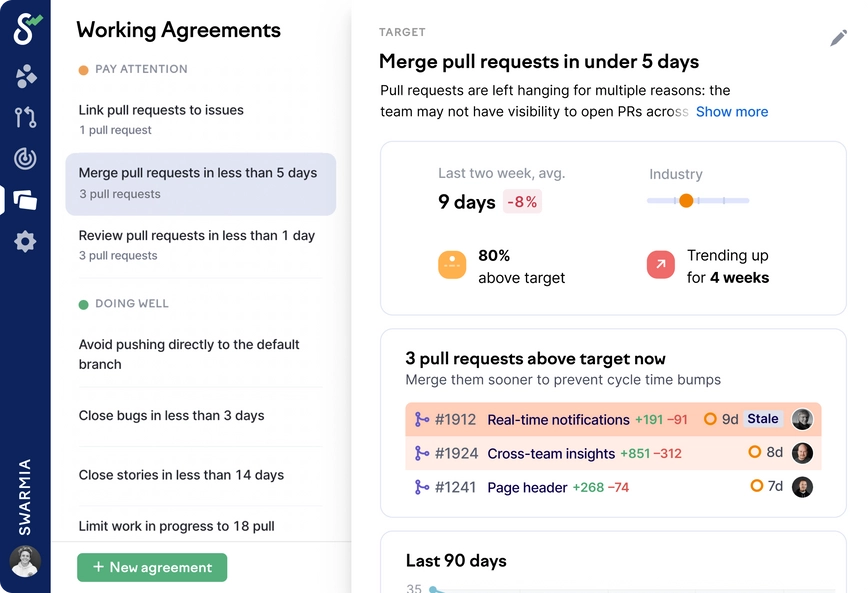
\includegraphics[width=13.5cm]{LaTeX/images/improvement.png}
        \caption{Working Agreements in Swarmia. On the left, a list of currently configured WAs. On the right, a detail view of a selected WA with WA-specific statistics.}
        \label{fig:WorkingAgreementsView}
    \end{center}
\end{figure}

The minimum number of individual contributors on a single issue tracker ticket is tracked with min\_issue\_contributors. Using this WA teams encourage working as a team to avoid siloing. To bridge the gap between version control and issue tracker data, teams can configure pull\_request\_linking, which ensures that all PRs are accompanied with a related issue tracker identifier.

The Working Agreement view in Swarmia is shown in Figure~\ref{fig:WorkingAgreementsView}. All team members can use this view to set and review WAs for their team. In the list left of page, current WAs and their status is shown. On the right a detail view of a WA, in this case max\_pull\_request\_age, is shown. In this view the user can access the current configuration and statistics, as well as see the items not within the target. 

\section{Data}

The data collected by Swarmia includes, but is not limited to, pull requests, issues, and failed deployments. Furthermore, Swarmia has read-only access to the source code, which is used to estimate the complexity of the change in question. Swarmia never stores client code but instead calculates the size of the change bundle and stores it in a separate database.

\begin{table}
\begin{center}
\begin{tabularx}{\textwidth}{|l|l|} 
\hline
parameter & description\\ [0.5ex] 
\hline\hline
wip\_pull\_requests & WA status \\
max\_pull\_request\_age & WA status \\
no\_direct\_pushes\_to\_main\_branch & WA status \\
min\_issue\_contributors  & WA status \\
wip\_issues & WA status \\
max\_issue\_age  & WA status \\
max\_pull\_request\_review\_time  & WA status \\
pull\_request\_linking  & WA status \\
github\_authors & Pull request authors \\
swarmia\_users & MAU in Swarmia team \\
slack\_users & Swarmia users with Slack notifications \\
daily\_digest & team's Slack daily digest status \\
target\_days & numeric target for a given WA \\
days\_in\_use & days since WA configuration \\
target\_achieved & whether target was achieved \\
ct\_days  & normalized cycle time in days \\

\hline
\end{tabularx}
\caption{Variables used in the study}
\label{tab:variables}
\end{center}
\end{table}




Processing of the data is done in Google's BigQuery data warehouse service. All data was processed according to the Swarmia privacy policies, including handling all the data with Swarmia managed devices. All aggregate data was removed at the end of the research.

\begin{figure}[ht]
\centering
\begin{tikzpicture}[
    every node/.style={align=center, minimum height=1em, minimum width=1cm,node distance=0.7cm},
]

%Nodes
\node[entity]      (teamswa)        {active teams with WA adoption};
\node[entity]      (teams)          [above=of teamswa] {team basic info};
\node[entity]      (snapshots)       [left=of teams] {team snapshots};
\node[entity]       (mau)           [right=of teams] {MAU};
\node[entity]      (ctwa)       [below=of teamswa] {cycle times with WA adoption};
\node[entity]      (cycletimes)       [left=of ctwa]     {cycle times};
\node[entity]      (adoption)       [left=of snapshots] {WA adoption};
\node[entity, fill=gray!20]       (lm)        [below=of ctwa] {linear model input data};

%Lines
\draw[->] (cycletimes.east) -- (ctwa.west);
\draw[->] (ctwa.south) -- (lm.north);
\draw[->] (teamswa.south) -- (ctwa.north);
\draw[->] (teams.south) -- (teamswa.north);
\draw[->] (snapshots.south) -- (teamswa.north);
\draw[->] (mau.south) -- (teamswa.north);
\draw[->] (adoption.south) -- (teamswa.north);

\end{tikzpicture}
\caption{Data flow in BigQuery}
\label{fig:dataFlow}
\end{figure}

Most of the information needed is already collected at Swarmia for business intelligence purposes but needs to be structured in a suitable format. The way raw data was combined into this format is shown in Figure~\ref{fig:dataFlow}. Additionally, for the needs of this study, weekly aggregates of team metrics were exported from the Swarmia application backend to BigQuery. This data set is called ``cycle times'' in Figure~\ref{fig:dataFlow}. These metrics were merged with basic team information, working agreement usage, and team member activity. Finally, team identifiers and timestamps were removed so the data points would be independent. A sample of the resulting data is displayed in Table~\ref{tab:dataExample}. All variables used in the study are listed in Table~\ref{tab:variables}.


\newcommand*\rot{\rotatebox{90}}
\begin{table}[ht]
\begin{center}
\begin{tabular}{|c|c|c|c|c|c|c|c|c|c|c|c|c|c|} 
\hline

No & A & B & C & D & E & F & G & H & ct\_days & slack\_users & daily\_digest \\ [0.5ex]
\hline\hline

1 & 0 & 1 & 0 & 0 & 0 & 0 & 1 & 0 & 1.3 & 2 & 0 \\
2 & 0 & 1 & 0 & 0 & 0 & 0 & 0 & 1 & 0.00031 & 0 & 0 \\ 
3 & 1 & 0 & 1 & 0 & 0 & 0 & 1 & 0 & -0.46 & 4 & 1 \\
4 & 0 & 0 & 0 & 0 & 0 & 0 & 0 & 1 & -0.058 & 5 & 1 \\
5 & 0 & 1 & 1 & 0 & 1 & 1 & 1 & 1 & -1.8 & null & 1 \\

\hline
\end{tabular}
\caption{Sample rows of lm\_data}
\label{tab:dataExample}
\end{center}
\end{table}


\section{Research Questions}

The first research question of this study is how teams use Working Agreements: more specifically, which share of Swarmia teams use each agreement and how these teams have configured their Working Agreements setup. 

The second research question is what is the effect of Working Agreements on software development cycle times. The hypothesis based on previous research (e.g.~\cite{stray_exploring_2016,teh_social_2012,forsgren_space_2021}) is that as Working Agreements promote methods that accelerate software development, they should directly impact the team's performance. We will look into the Working Agreement composition in different teams and determine which agreements impact the teams' cycle times most. 

\section{Approach}

To answer RQ1, data from Swarmia is used to determine how many of the teams have enabled which Working Agreements. Furthermore, we look into how many Working Agreements teams usually use and what goals they have configured for the WAs. For example, WIP limit agreements require teams to specify a threshold for open items. Lastly, team characteristics, such as team size, and their connection to the Working Agreements setup, are analyzed. Some Working Agreements can be configured multiple times for different issue types. The way teams configure these issue-related WAs is further investigated.  

Data from all teams using the Working Agreements feature is collected and analyzed to help answer RQ2. Historical activity data is pulled from the teams' source control repositories from 1 July 2020 to 31 July 2022. The data is aggregated weekly for 24 months: some teams have been clients for longer than two years, and some for a shorter amount. All teams included in the study had at least two months of data. The variability of the data collection period should be acceptable, as averages are used, and the period length is not a variable in the analysis.

\begin{figure}[ht]
    \begin{center}
        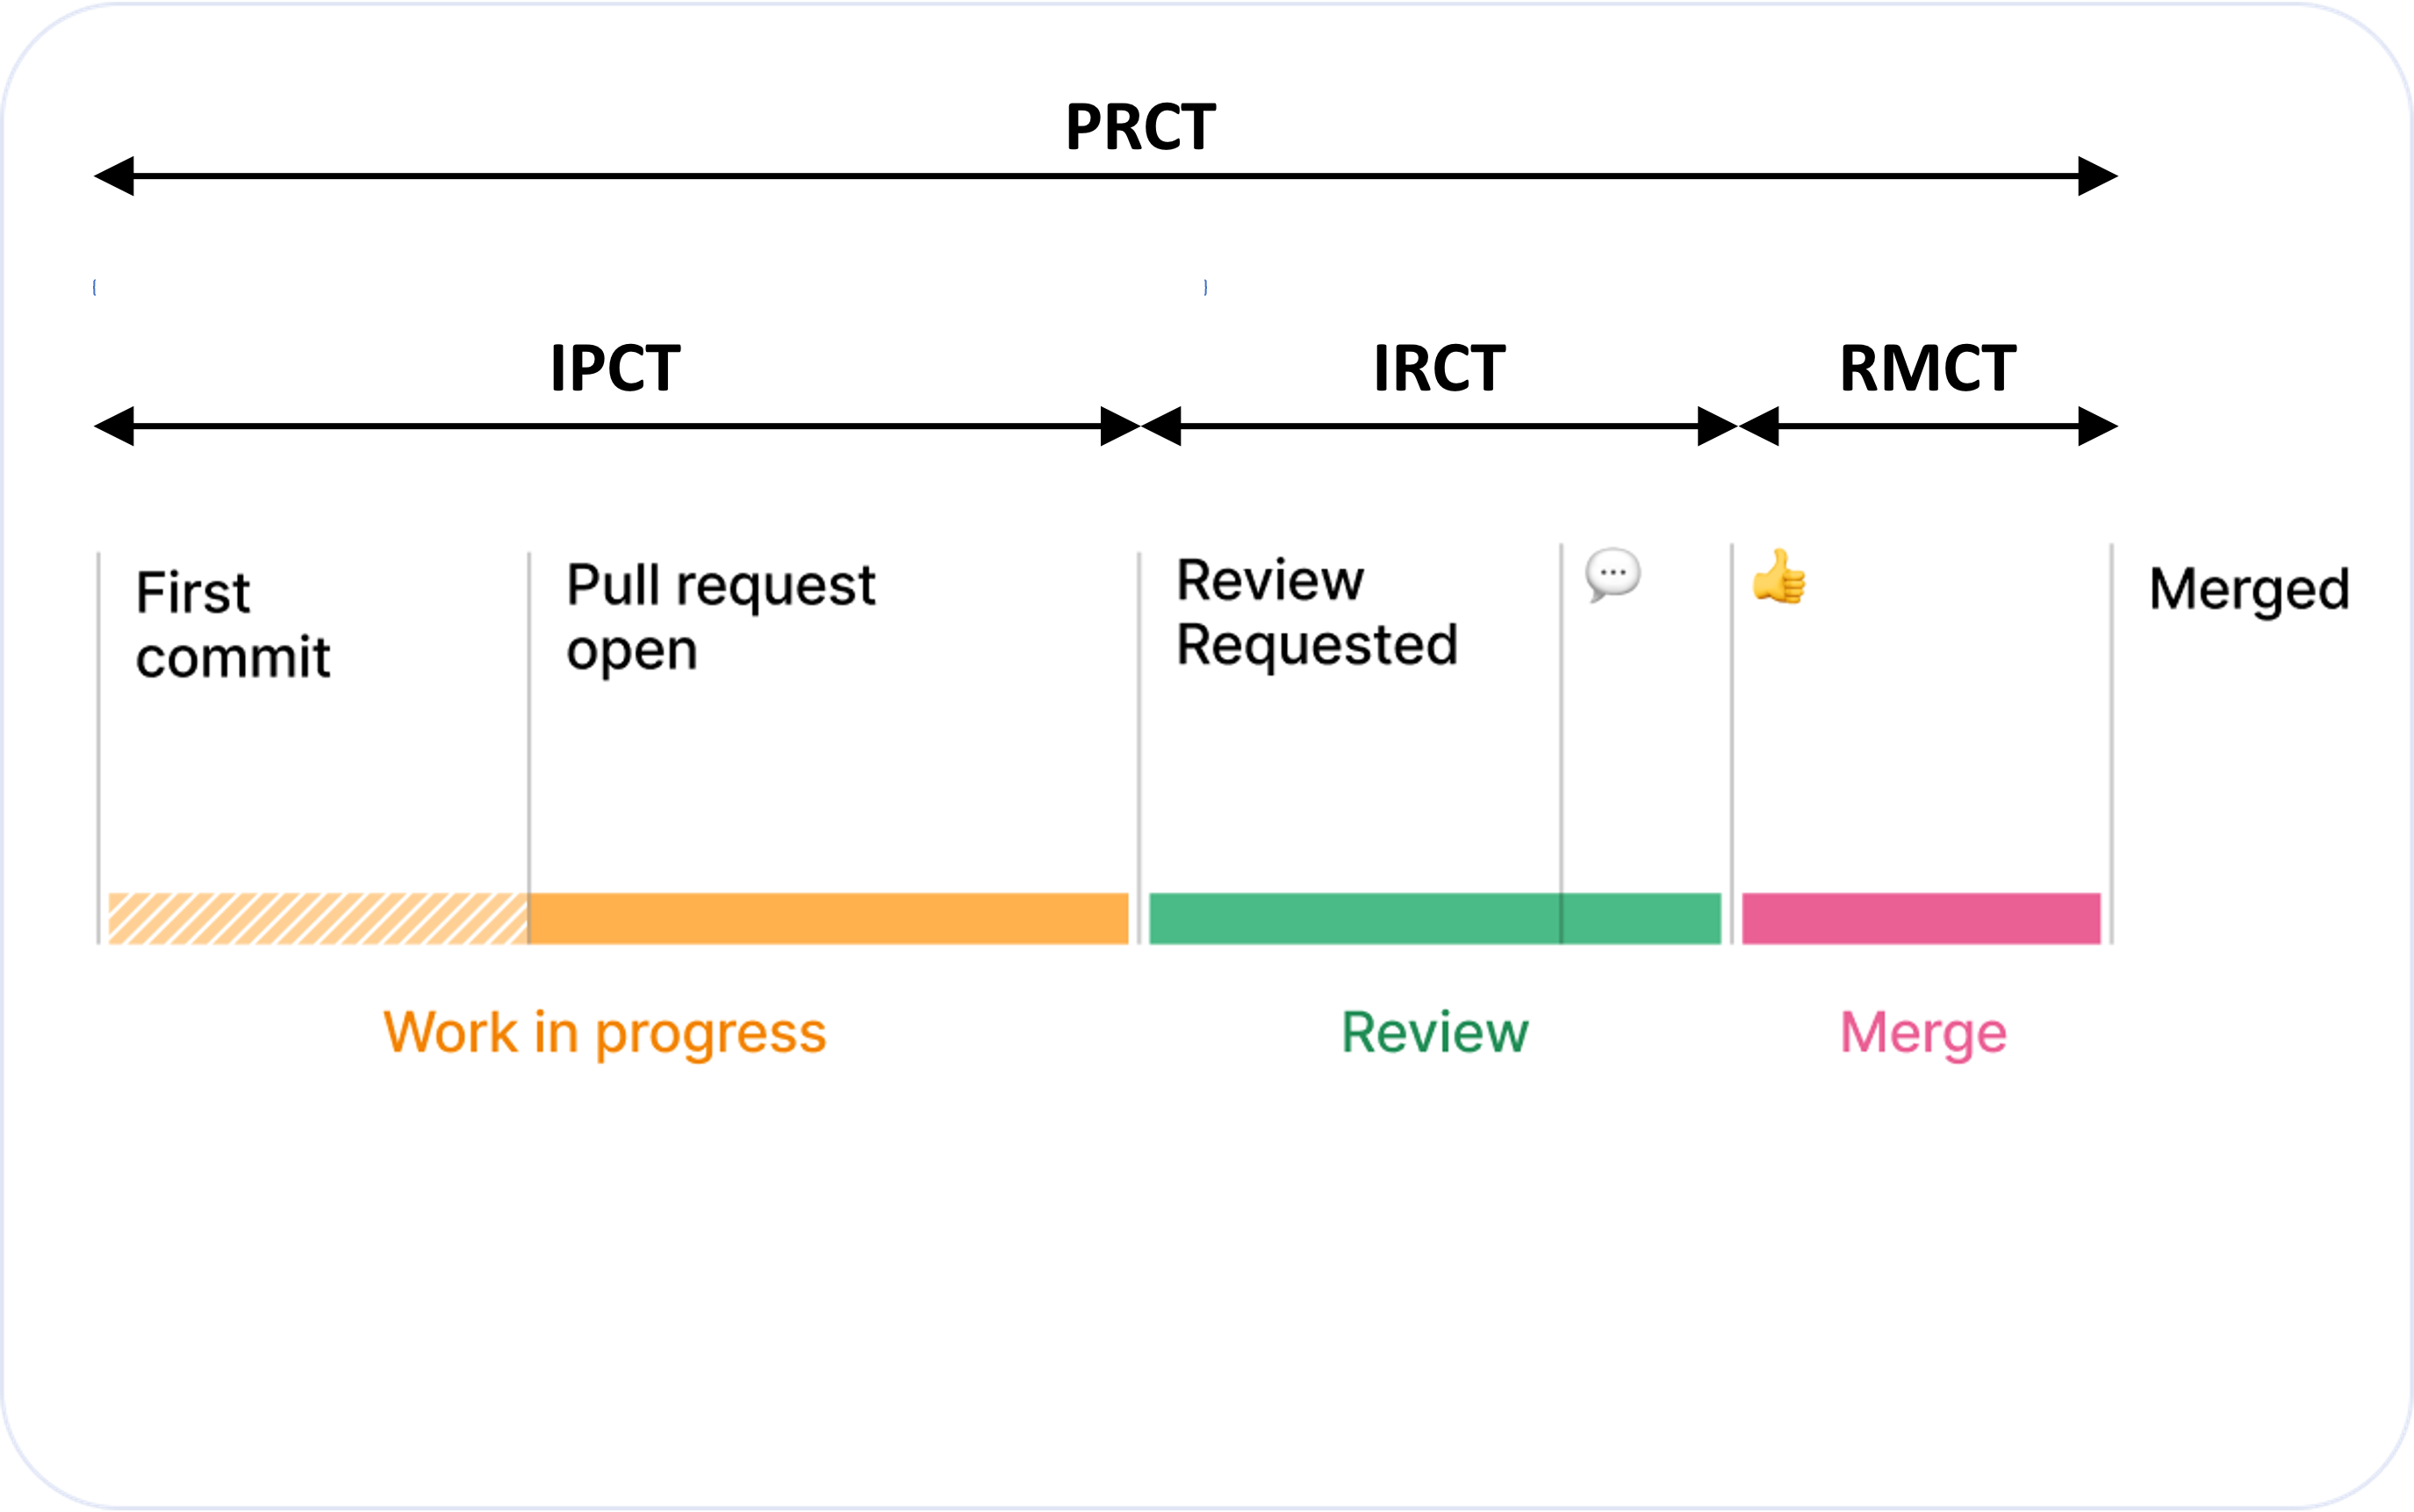
\includegraphics[width=13.5cm]{LaTeX/images/cts-defined-arrows.png}
        \caption{Cycle time definitions}
        \label{fig:ctsArrows}
    \end{center}
\end{figure}

The key metric used in the analysis is the Pull Request Cycle Time (PRCT). Additionally, we look into the sub-parts of PRCT: In Progress Cycle Time (IPCT), In Review Cycle Time (IRCT), and Ready to Merge Cycle Time (RMCT). The span of these metrics in relation to each other is shown in Figure~\ref{fig:ctsArrows}. 

Even though Swarmia exports data from issue trackers, these data sources were left out of the analysis based on the scope of the thesis. The analysis is done in BigQuery in line with Swarmia's privacy policy. In addition to a standard SQL query engine, BigQuery offers advanced data analysis capabilities. For this thesis, the inbuilt linear regression feature was utilized. Figure~\ref{fig:dataFlow} presents the data flow before building the regression model. 

We look at the relationship between the independent and dependent variables in linear regression. The dependent variable is the one that, as a hypothesis, depends on the values of the independent variables. Respectively, the independent variables are the configuration of Working Agreements, team member metrics, and Slack notification settings. 

\definecolor{cor-very-weak}{HTML}{BBBBBB}
\definecolor{cor-weak}{HTML}{EEBD84}
\definecolor{cor-moderate}{HTML}{F47461}
\definecolor{cor-strong}{HTML}{F47461}
\definecolor{cor-very-strong}{HTML}{8B0000}

\begin{table}[ht]
\centering
\resizebox{\columnwidth}{!}{
\begin{tabular}{c c c c c c c c c c c c c}

& A & B & C & D & E & F & G & H & ga & sw & sl & dd\\ \hline
A & \textcolor{cor-very-strong}{1.0} & \textcolor{cor-moderate}{0.49} & \textcolor{cor-weak}{0.28} & \textcolor{cor-very-weak}{0.16} & \textcolor{cor-weak}{0.29} & \textcolor{cor-very-weak}{0.15} & \textcolor{cor-moderate}{0.42} & \textcolor{cor-weak}{0.24} & \textcolor{cor-very-weak}{-0.09} & \textcolor{cor-very-weak}{-0.04} & \textcolor{cor-very-weak}{-0.03} & \textcolor{cor-weak}{0.2}\\ \hline
B &  & \textcolor{cor-very-strong}{1.0} & \textcolor{cor-weak}{0.23} & \textcolor{cor-very-weak}{0.18} & \textcolor{cor-weak}{0.32} & \textcolor{cor-weak}{0.31} & \textcolor{cor-strong}{0.64} & \textcolor{cor-weak}{0.39} & \textcolor{cor-very-weak}{-0.07} & \textcolor{cor-very-weak}{0.02} & \textcolor{cor-very-weak}{0.06} & \textcolor{cor-weak}{0.23}\\ \hline
C &  &  & \textcolor{cor-very-strong}{1.0} & \textcolor{cor-weak}{0.25} & \textcolor{cor-weak}{0.26} & \textcolor{cor-very-weak}{0.16} & \textcolor{cor-weak}{0.24} & \textcolor{cor-weak}{0.35} & \textcolor{cor-very-weak}{-0.1} & \textcolor{cor-very-weak}{0.0} & \textcolor{cor-very-weak}{-0.06} & \textcolor{cor-very-weak}{0.09}\\ \hline
D &  &  &  & \textcolor{cor-very-strong}{1.0} & \textcolor{cor-weak}{0.3} & \textcolor{cor-weak}{0.25} & \textcolor{cor-very-weak}{0.15} & \textcolor{cor-weak}{0.3} & \textcolor{cor-very-weak}{0.03} & \textcolor{cor-very-weak}{0.09} & \textcolor{cor-very-weak}{0.0} & \textcolor{cor-very-weak}{0.03}\\ \hline
E &  &  &  &  & \textcolor{cor-very-strong}{1.0} & \textcolor{cor-moderate}{0.58} & \textcolor{cor-weak}{0.28} & \textcolor{cor-moderate}{0.43} & \textcolor{cor-very-weak}{-0.09} & \textcolor{cor-very-weak}{0.01} & \textcolor{cor-very-weak}{-0.02} & \textcolor{cor-very-weak}{0.15}\\ \hline
F &  &  &  &  &  & \textcolor{cor-very-strong}{1.0} & \textcolor{cor-weak}{0.32} & \textcolor{cor-weak}{0.34} & \textcolor{cor-very-weak}{-0.03} & \textcolor{cor-very-weak}{0.08} & \textcolor{cor-very-weak}{0.05} & \textcolor{cor-very-weak}{0.19}\\ \hline
G &  &  &  &  &  &  & \textcolor{cor-very-strong}{1.0} & \textcolor{cor-weak}{0.3} & \textcolor{cor-very-weak}{-0.01} & \textcolor{cor-very-weak}{0.03} & \textcolor{cor-very-weak}{0.08} & \textcolor{cor-weak}{0.32}\\ \hline
H &  &  &  &  &  &  &  & \textcolor{cor-very-strong}{1.0} & \textcolor{cor-very-weak}{-0.09} & \textcolor{cor-very-weak}{0.0} & \textcolor{cor-very-weak}{-0.01} & \textcolor{cor-very-weak}{0.1}\\ \hline
ga &  &  &  &  &  &  &  &  & \textcolor{cor-very-strong}{1.0} & \textcolor{cor-strong}{0.79} & \textcolor{cor-strong}{0.78} & \textcolor{cor-very-weak}{-0.18}\\ \hline
sw &  &  &  &  &  &  &  &  &  & \textcolor{cor-very-strong}{1.0} & \textcolor{cor-very-strong}{0.84} & \textcolor{cor-very-weak}{-0.07}\\ \hline
sl &  &  &  &  &  &  &  &  &  &  & \textcolor{cor-very-strong}{1.0} & \textcolor{cor-very-weak}{-0.01}\\ \hline
dd &  &  &  &  &  &  &  &  &  &  &  & \textcolor{cor-very-strong}{1.0}\\ \hline

\end{tabular}
}

\caption{Correlation matrix. The stronger the correlation, the darker the color. ga=github\_authors, sw=swarmia\_users, sl=slack\_users, dd=daily\_digest}
\label{tab:correlationMatrix}
\end{table}

Pearson correlation coefficient for independent variables is calculated in Table~\ref{tab:correlationMatrix} to ensure the data is compatible with linear regression analysis: two variables should not correlate for the model to work as expected. The most considerable correlation encountered is the of slack\_users and swarmia\_users with a value of 0.84. The pairs with high correlation deal with the same themes, for example, WAs related to pull requests. Even though some of the WAs correlate, the data can be used for the model with slight modifications: github\_authors and swarmia\_users were dropped to include only the team member metric, slack\_users. 

\begin{samepage}

Linear regression can be formulated as follows:
\begin{equation}
Y = \beta_0 + \beta_i X_i + \beta_{i+1} X_{i+1} + \ldots + \beta_n X_n + \epsilon
\end{equation}

where
\begin{description}
\item $Y$ is dependent variable
\item $\beta_0$ is the constant coefficient (intercept)
\item $\beta_i$ is slope for $X_i$
\item $X_i$ is independent variable
\item $\epsilon$ is error
\end{description}

\end{samepage}

The training data is passed to linear regression models in a form presented in Table~\ref{tab:dataExample}. The data has gone through two significant modifications to suit linear regression. First, we calculated each team's average cycle times before enabling any Working Agreements. This average is then subtracted from each data point's cycle time to achieve a normalized data set: the aim is to diminish the differences between teams to achieve comparable cycle times. Secondly, WA activation dates are mapped to Boolean values for each row: the value is zero if WA has not been activated yet and one if it has.

At the beginning of the analysis, three team member-related metrics were included: github\_authors, swarmia\_users, and slack\_users. The amount of Swarmia users did not have statistical significance and strongly correlated with github\_authors with a correlation of $0.79$. In the end, out of the three metrics, only slack\_users was retained in the final model.

The targets set for agreements max\_pull\_request\_age and max\_pull\_re\-quest\_re\-view\_time were studied with dedicated models. These target models use a Boolean independent variable, calculated from $cycletime<target$. The dependent variables in these models are daily\_digest, slack\_users, days\_in\_use: the days the WA has been in use, and tar\-get\_days: the set target for the given WA. A sample of data used in these models is shown in Table~\ref{tab:targetData}.

\begin{table}[ht]
\begin{center}
\begin{tabular}{|c|c|c|c|c|} 
\hline

daily\_digest & slack\_users & days\_in\_use & target\_days & target\_achieved  \\ [0.5ex]
\hline\hline

1 & 22 & 514 & 3.0 & 1 \\
1 & 8 & 166 & 7.0 & 1 \\
1 & 1 & 70 & 14.0 & 0 \\
1 & 3 & 40 & 3.0 & 0 \\
0 & 10 & 132 & 7.0 & 1 \\

\hline
\end{tabular}
\caption{Sample rows of target model input data}
\label{tab:targetData}
\end{center}
\end{table}


The threshold value $\alpha$ selected for the study diverts from the standard convention of $\alpha=0.05$. Instead, results with a p-value of $p<0.10$ are considered as having statistical significance against the null hypothesis. Furthermore, results with a p-value of $p<0.05$ and $p<0.01$ were given additional noteworthiness. These three categories of significance are denoted with asterisks in figures and tables. All results are reported with a the precision of three significant figures.

In the analysis, p-values are considered as one factor that contributes to the reliability of the findings. When interpreting the findings, we rely on the weights of the independent variables of the linear model for further evidence. We note that the results are exploratory and future research should explore similar phenomena in other contexts.